\documentclass[border=10pt]{standalone}
\usepackage{tikz}
\usepackage{xcolor}
\usetikzlibrary{shapes,arrows.meta,positioning,calc,shadows,backgrounds,fit}

% Colors
\definecolor{researchblue}{RGB}{41,128,185}
\definecolor{translationpurple}{RGB}{142,68,173}
\definecolor{prototypegreen}{RGB}{39,174,96}
\definecolor{validationorange}{RGB}{230,126,34}
\definecolor{productionred}{RGB}{192,57,43}
\definecolor{lightgray}{RGB}{245,245,245}
\definecolor{darktext}{RGB}{50,50,50}

\begin{document}
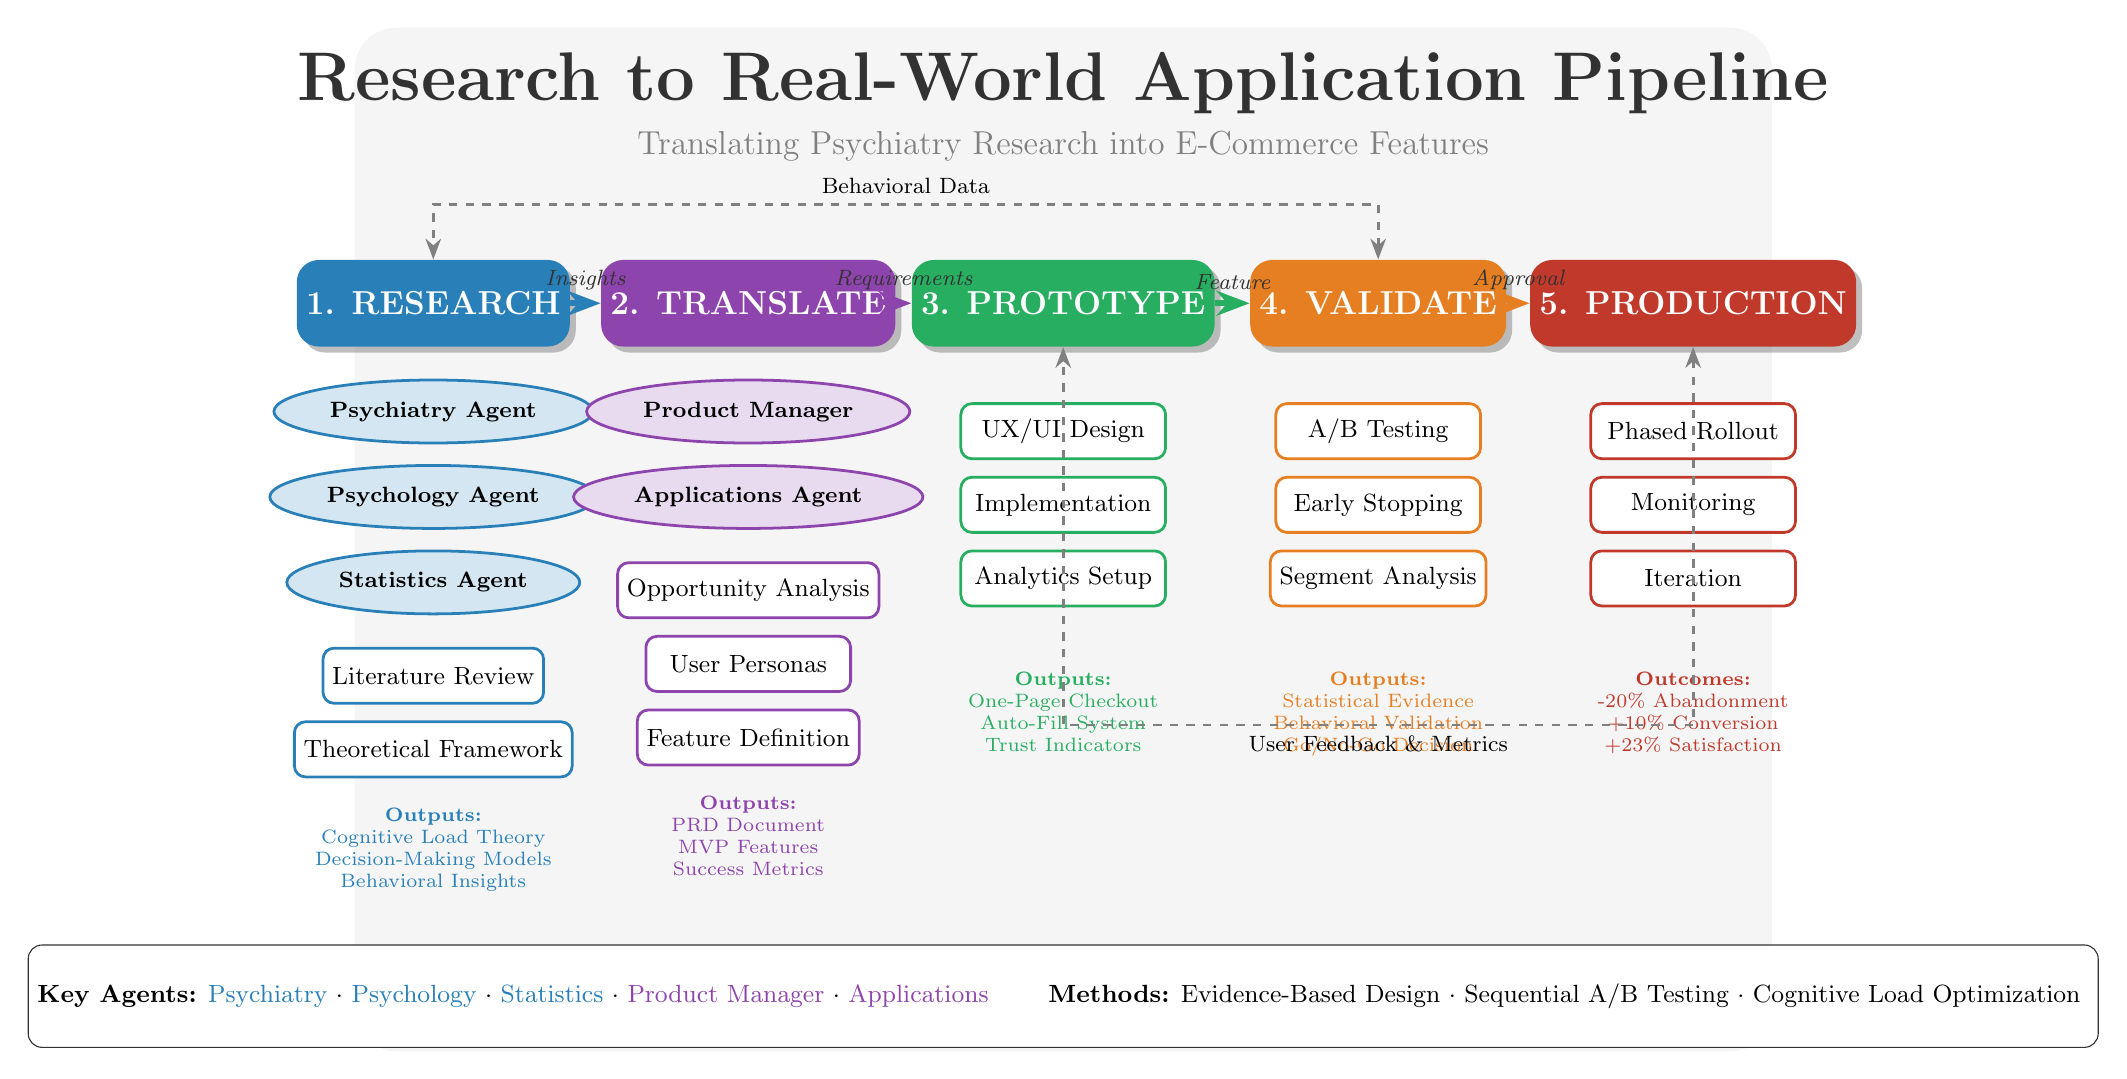
\begin{tikzpicture}[
    % Node styles
    phase/.style={
        rectangle,
        rounded corners=8pt,
        minimum width=3.2cm,
        minimum height=1.1cm,
        text centered,
        font=\bfseries\large,
        text=white,
        drop shadow
    },
    subnode/.style={
        rectangle,
        rounded corners=4pt,
        minimum width=2.6cm,
        minimum height=0.7cm,
        text centered,
        font=\small,
        fill=white,
        draw=#1,
        line width=1pt
    },
    agent/.style={
        ellipse,
        minimum width=2.4cm,
        minimum height=0.8cm,
        text centered,
        font=\footnotesize\bfseries,
        fill=#1!20,
        draw=#1,
        line width=1pt
    },
    arrow/.style={
        ->,
        >=Stealth,
        line width=2pt,
        draw=darktext
    },
    feedback/.style={
        <->,
        >=Stealth,
        line width=1pt,
        draw=gray,
        dashed
    },
    label/.style={
        font=\footnotesize\itshape,
        text=darktext
    }
]

% Background
\begin{scope}[on background layer]
    \fill[lightgray, rounded corners=15pt] (-1,-8.5) rectangle (17,4.5);
\end{scope}

% Title
\node[font=\Huge\bfseries, text=darktext] at (8,3.8) {Research to Real-World Application Pipeline};
\node[font=\large, text=gray] at (8,3) {Translating Psychiatry Research into E-Commerce Features};

%==============================================================================
% PHASE 1: RESEARCH
%==============================================================================
\node[phase, fill=researchblue] (research) at (0,1) {1. RESEARCH};

\node[agent=researchblue, below=0.4cm of research] (psychiatry) {Psychiatry Agent};
\node[agent=researchblue, below=0.25cm of psychiatry] (psychology) {Psychology Agent};
\node[agent=researchblue, below=0.25cm of psychology] (stats) {Statistics Agent};

\node[subnode=researchblue, below=0.4cm of stats] (lit) {Literature Review};
\node[subnode=researchblue, below=0.2cm of lit] (theory) {Theoretical Framework};

% Research outputs
\node[font=\scriptsize, text=researchblue, below=0.25cm of theory, align=center] (research_out) {
    \textbf{Outputs:}\\
    Cognitive Load Theory\\
    Decision-Making Models\\
    Behavioral Insights
};

%==============================================================================
% PHASE 2: TRANSLATION
%==============================================================================
\node[phase, fill=translationpurple] (translate) at (4,1) {2. TRANSLATE};

\node[agent=translationpurple, below=0.4cm of translate] (pm) {Product Manager};
\node[agent=translationpurple, below=0.25cm of pm] (apps) {Applications Agent};

\node[subnode=translationpurple, below=0.4cm of apps] (opp) {Opportunity Analysis};
\node[subnode=translationpurple, below=0.2cm of opp] (persona) {User Personas};
\node[subnode=translationpurple, below=0.2cm of persona] (features) {Feature Definition};

% Translation outputs
\node[font=\scriptsize, text=translationpurple, below=0.25cm of features, align=center] (trans_out) {
    \textbf{Outputs:}\\
    PRD Document\\
    MVP Features\\
    Success Metrics
};

%==============================================================================
% PHASE 3: PROTOTYPE
%==============================================================================
\node[phase, fill=prototypegreen] (prototype) at (8,1) {3. PROTOTYPE};

\node[subnode=prototypegreen, below=0.7cm of prototype] (design) {UX/UI Design};
\node[subnode=prototypegreen, below=0.2cm of design] (impl) {Implementation};
\node[subnode=prototypegreen, below=0.2cm of impl] (analytics) {Analytics Setup};

% Prototype outputs
\node[font=\scriptsize, text=prototypegreen, below=0.7cm of analytics, align=center] (proto_out) {
    \textbf{Outputs:}\\
    One-Page Checkout\\
    Auto-Fill System\\
    Trust Indicators
};

%==============================================================================
% PHASE 4: VALIDATION
%==============================================================================
\node[phase, fill=validationorange] (validate) at (12,1) {4. VALIDATE};

\node[subnode=validationorange, below=0.7cm of validate] (ab) {A/B Testing};
\node[subnode=validationorange, below=0.2cm of ab] (early) {Early Stopping};
\node[subnode=validationorange, below=0.2cm of early] (segment) {Segment Analysis};

% Validation outputs
\node[font=\scriptsize, text=validationorange, below=0.7cm of segment, align=center] (val_out) {
    \textbf{Outputs:}\\
    Statistical Evidence\\
    Behavioral Validation\\
    Go/No-Go Decision
};

%==============================================================================
% PHASE 5: PRODUCTION
%==============================================================================
\node[phase, fill=productionred] (production) at (16,1) {5. PRODUCTION};

\node[subnode=productionred, below=0.7cm of production] (rollout) {Phased Rollout};
\node[subnode=productionred, below=0.2cm of rollout] (monitor) {Monitoring};
\node[subnode=productionred, below=0.2cm of monitor] (iterate) {Iteration};

% Production outputs
\node[font=\scriptsize, text=productionred, below=0.7cm of iterate, align=center] (prod_out) {
    \textbf{Outcomes:}\\
    -20\% Abandonment\\
    +10\% Conversion\\
    +23\% Satisfaction
};

%==============================================================================
% MAIN FLOW ARROWS
%==============================================================================
\draw[arrow, draw=researchblue] (research.east) -- (translate.west);
\draw[arrow, draw=translationpurple] (translate.east) -- (prototype.west);
\draw[arrow, draw=prototypegreen] (prototype.east) -- (validate.west);
\draw[arrow, draw=validationorange] (validate.east) -- (production.west);

% Arrow labels
\node[label, above=0.05cm] at ($(research.east)!0.5!(translate.west)$) {Insights};
\node[label, above=0.05cm] at ($(translate.east)!0.5!(prototype.west)$) {Requirements};
\node[label, above=0.05cm] at ($(prototype.east)!0.5!(validate.west)$) {Feature};
\node[label, above=0.05cm] at ($(validate.east)!0.5!(production.west)$) {Approval};

%==============================================================================
% FEEDBACK LOOPS
%==============================================================================
% Validation to Research feedback
\draw[feedback]
    (validate.north) -- ++(0,0.7) -|
    node[pos=0.25, above, font=\footnotesize] {Behavioral Data}
    (research.north);

% Production to Prototype feedback
\draw[feedback]
    (production.south) -- ++(0,-4.8) -|
    node[pos=0.25, below, font=\footnotesize] {User Feedback \& Metrics}
    (prototype.south);

%==============================================================================
% KEY COMPONENTS BOX
%==============================================================================
\node[draw=darktext, rounded corners=5pt, fill=white,
      minimum width=15cm, minimum height=1.3cm,
      font=\small, align=center] at (8,-7.8) {
    \textbf{Key Agents:}
    \textcolor{researchblue}{Psychiatry} $\cdot$
    \textcolor{researchblue}{Psychology} $\cdot$
    \textcolor{researchblue}{Statistics} $\cdot$
    \textcolor{translationpurple}{Product Manager} $\cdot$
    \textcolor{translationpurple}{Applications}
    \quad\quad
    \textbf{Methods:}
    Evidence-Based Design $\cdot$ Sequential A/B Testing $\cdot$ Cognitive Load Optimization
};

\end{tikzpicture}
\end{document}
